% =====================================================================
% Snippet: line-chart.tex
% =====================================================================
% USAGE: Line chart with 1-2 curves (e.g., training loss, accuracy
% over epochs). Includes axes, gridlines, optional smoothed curve.
% Used in examples 08 Diffusion (Training Loss Curve panel).
%
% Copy %% COPY-START / END, replace:
%   - data1, data2: comma-separated "x/y" pairs
%   - x_max, y_max: axis limits
%   - title, x_label, y_label
%   - chart_W, chart_H: plot area
% =====================================================================

\documentclass[tikz,border=10pt]{standalone}
\usepackage{xcolor,tikz}
\usetikzlibrary{positioning,calc}

\definecolor{acaRedLine}{HTML}{C03030}
\definecolor{acaBlueLine}{HTML}{3060A8}
\definecolor{acaGreenLine}{HTML}{389050}
\definecolor{acaGreyLine}{HTML}{606060}

\begin{document}
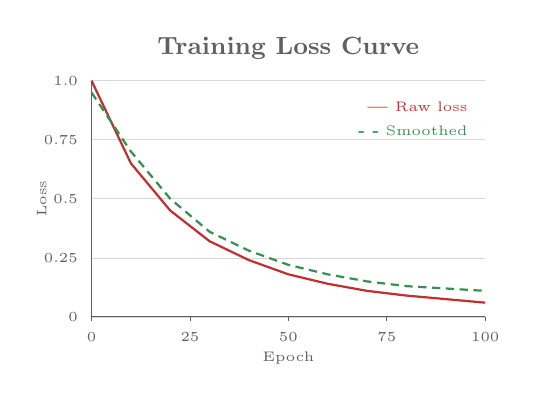
\begin{tikzpicture}

%% COPY-START =========================================================

% --- DATA (replace with your actual values) ---
% Raw loss (decaying exponential)
\def\dataRaw{0/1.0, 10/0.65, 20/0.45, 30/0.32, 40/0.24,
             50/0.18, 60/0.14, 70/0.11, 80/0.09, 90/0.075, 100/0.06}
% Smoothed/validation loss
\def\dataSmooth{0/0.95, 10/0.70, 20/0.50, 30/0.36, 40/0.28,
                50/0.22, 60/0.18, 70/0.15, 80/0.13, 90/0.12, 100/0.11}

\def\xO{0}
\def\yO{0}
\def\chartW{5.0}
\def\chartH{3.0}
\def\xMax{100}
\def\yMax{1.0}

% --- AXES ---
\draw[acaGreyLine, line width=0.5pt]
  (\xO, \yO) -- (\xO + \chartW, \yO);
\draw[acaGreyLine, line width=0.5pt]
  (\xO, \yO) -- (\xO, \yO + \chartH);

% --- GRIDLINES + Y-TICKS ---
\foreach \pct in {0, 0.25, 0.5, 0.75, 1.0} {
  \pgfmathsetmacro\ypos{\yO + \chartH * \pct}
  \draw[acaGreyLine!25, line width=0.2pt]
    (\xO, \ypos) -- (\xO + \chartW, \ypos);
  \node[anchor=east, font=\tiny, color=acaGreyLine]
    at (\xO - 0.05, \ypos) {\pct};
}

% --- X-TICKS ---
\foreach \xv in {0, 25, 50, 75, 100} {
  \pgfmathsetmacro\xpos{\xO + \chartW * \xv / \xMax}
  \draw[acaGreyLine, line width=0.3pt]
    (\xpos, \yO) -- (\xpos, \yO - 0.05);
  \node[anchor=north, font=\tiny, color=acaGreyLine]
    at (\xpos, \yO - 0.08) {\xv};
}

% --- CURVE 1: Raw loss (red) ---
% Note: cannot use \foreach inside plot coordinates {}.
% Build path manually by computing coords + chaining with `--`.
\foreach \xv/\yv [count=\i] in \dataRaw {
  \pgfmathsetmacro\px{\xO + \chartW * \xv / \xMax}
  \pgfmathsetmacro\py{\yO + \chartH * \yv / \yMax}
  \coordinate (raw\i) at (\px, \py);
}
\draw[acaRedLine, line width=0.8pt]
  (raw1) -- (raw2) -- (raw3) -- (raw4) -- (raw5) -- (raw6)
  -- (raw7) -- (raw8) -- (raw9) -- (raw10) -- (raw11);

% --- CURVE 2: Smoothed (green dashed) ---
\foreach \xv/\yv [count=\i] in \dataSmooth {
  \pgfmathsetmacro\px{\xO + \chartW * \xv / \xMax}
  \pgfmathsetmacro\py{\yO + \chartH * \yv / \yMax}
  \coordinate (sm\i) at (\px, \py);
}
\draw[acaGreenLine, line width=0.8pt, densely dashed]
  (sm1) -- (sm2) -- (sm3) -- (sm4) -- (sm5) -- (sm6)
  -- (sm7) -- (sm8) -- (sm9) -- (sm10) -- (sm11);

% --- LEGEND (top right) ---
\node[anchor=north east, font=\tiny, color=acaRedLine]
  at (\xO + \chartW - 0.1, \yO + \chartH - 0.15)
  {\textbf{---} Raw loss};
\node[anchor=north east, font=\tiny, color=acaGreenLine]
  at (\xO + \chartW - 0.1, \yO + \chartH - 0.45)
  {\textbf{- -} Smoothed};

% --- LABELS ---
\node[anchor=north, font=\tiny, color=acaGreyLine]
  at (\xO + \chartW/2, \yO - 0.32) {Epoch};
\node[anchor=south, font=\tiny, color=acaGreyLine, rotate=90]
  at (\xO - 0.45, \yO + \chartH/2) {Loss};
\node[anchor=south, font=\small\bfseries, color=acaGreyLine]
  at (\xO + \chartW/2, \yO + \chartH + 0.15) {Training Loss Curve};

%% COPY-END ===========================================================

\end{tikzpicture}
\end{document}
